\icode{N19Q-MD-SI-L2-261111-003}
\nceeID[unkown]{2019海南}{unkown}
如图，两物块 \(P\)、\(Q\) 置于水平地面上，其质量分别为 \(m\)、\(2m\)，两者之间用水平轻绳连接。两物块与地面之间的动摩擦因数均为 \(\mu\)，重力加速度大小为 \(g\)，现对 \(Q\) 施加一水平向右的拉力 \(F\)，使两物块做匀加速直线运动，轻绳的张力大小为\paren[]

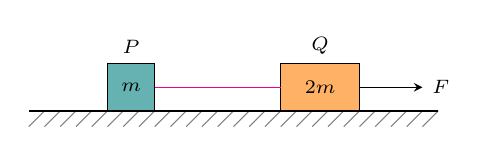
\begin{tikzpicture}[>=stealth,font=\scriptsize]
	\draw[fill=teal!60] (0,0) rectangle(.6,0.6)node[midway]{\(m\)};
	\draw[fill=orange!60] (3.2,0) rectangle(2.2,.6)node[midway]{\(2m\)};
	\draw[->] (3.2,.3)--(4,.3)node[right]{\(F\)};
	\draw[magenta] (.6,.3)--(2.2,.3);
	\node at(.3,.6)[above]{\(P\)};
	\node at(2.7,.6)[above]{\(Q\)};
	\foreach \x in {-1,-.8,...,4}
		\draw[gray] (\x,-.2)--++(.2,.2);
	\draw[thick] (-1,0)--(4.2,0);
\end{tikzpicture}
\begin{choices}
	\item \(F - 2\mu mg\)
	\item \(\dfrac{1}{3}F - \mu mg\)
	\item \(\dfrac{1}{3}F +\mu mg\)
	\item \(\dfrac{1}{3}F\)
\end{choices}
\begin{answer}
	D\qquad 提示：
\end{answer}